\documentclass{article}
\usepackage{graphicx}

\begin{document}
\title{Assignment 2: End to end machine learning project}
\author{Pravin Lamichhane}
\date{September 2025}
\maketitle
\section{Introduction}
This assignment intends to cover the end to end machine learning project life cycle and contains are refrenced from book Hands on Machine Learning .
1. Frame the problem.
2. Get the data.
3. Explore and visualize the data to gain insights.
4. Prepare the data for machine learning algorithms.
5. Select a model and train it.
6. Fine-tune your model.
7. Launch, monitor, and maintain your system.

\section{Frame the problem}
Initial step in machine learning project is to fram the problem statement or understand the objective , answer an organization/person is looking for . This step is crucial as it sets the direction for the entire project. A well-defined problem statement helps in identifying the right data, selecting appropriate algorithms, and evaluating the success of the model. For example, if the objective is to predict customer churn, the problem can be framed as a binary classification task where the goal is to classify customers into 'churn' or 'not churn' based on their behavior and attributes.
\section{Get the data}
Data is the foundation of any machine learning project. In this step relevant data is collected , real life machine learning problems often dont have readily available data 
and may require web scraping , using APIs or other data collection methods to grather the necessary information. 
Grathering of the data can be based on framming of the problem statement. For example , if the problem is to predict house prices , data can be collected from real estate websites or public datasets that contain information about house features and their corresponding prices. 
Data can be structured or unstructured , and it is important to ensure that the data is relevant, accurate, and sufficient for training the model.

\section{Explore and visualize the data to gain insights}
Once the data is collected , it is important to run an exploratory data analysis (EDA) to understand the structure, patterns, and relationships within the data. This step involves using statistical techniques and visualization tools to summarize the main characteristics of the data. Data sometime have missing values , outliers or inconsistencies that needs to be excluded or normalized before processing the data further . Visualization techiques as data distributon , corelation matrix can provide more inshights into data 
A model is as good as the data it is trained on , hence understanding the data is cruciual for building and machine learnging model.
\subsection{Processs , libraries used}
Data are typically stored in tabular format like csv files or relational databases. libraries like pandas are used to load and manipulate the data. Visualization libraries like matplotlib and seaborn are used to create plots and charts to visualize the data.
\subsection{data types}
Data can be of various types including numerical (continuous or discrete), categorical (nominal or ordinal), text, images, and time series. Each data type may require different preprocessing techniques and algorithms for analysis.
\section{Prepare the data for machine learning algorithms}
Cleaning the Data : This step involves handling missing values, removing duplicates, and correcting inconsistencies in the data. Techniques such as imputation, interpolation, and outlier detection can be used to clean the data.
Transforming the Data : This step involves scaling, normalizing, and encoding the data to make it suitable for machine learning algorithms. Techniques such as min-max scaling, z-score normalization, and one-hot encoding can be used to transform the data.
Splitting the Data : This step involves dividing the data into training, validation, and test sets
\section{Select a model and train it}
Once the data is prepared, the next step is to select an appropriate machine learning model based on the problem type (e.g., regression, classification, clustering) and the characteristics of the data. Common models include linear regression, logistic regression, decision trees, random forests, support vector machines.
Data is always split into training and testing sets. The training set is used to train the model, while the testing set is used to evaluate its performance. The model is trained by feeding the training data into the algorithm and adjusting its parameters to minimize the error between the predicted and actual values.
Test set is used to evaluate the model performance on unseen data. Common evaluation metrics include accuracy, precision, recall, F1-score for classification tasks, and mean squared error (MSE) or R-squared for regression tasks.
\section{Fine-tune your model}
Once the initial model is trained, it is important to fine-tune its hyperparameters to optimize its performance. This can be done using techniques such as cross-validation, grid search, and random search
to find the best combination of hyperparameters that yield the highest performance on the validation set.
Cross-validation involves splitting the training data into multiple folds and training the model on different combinations of folds to evaluate its performance. Grid search involves specifying a range of values for each hyperparameter and exhaustively searching through all possible combinations to find the best one. Random search involves randomly sampling hyperparameter values from a specified distribution to find the best combination.

\section{Launch, monitor, and maintain your system}
Once the model is fine-tuned and evaluated, it can be deployed into a production environment where it can make predictions on new data. This step involves integrating the model into an application or system that can use its predictions to make decisions or provide insights.
Monitoring the model's performance in production is crucial to ensure that it continues to perform well over time. This can be done by tracking key metrics such as accuracy, precision, recall, and F1-score, and comparing them to the performance on the validation set. If the model's performance degrades over time, it may be necessary to retrain the model with new data or fine-tune its hyperparameters.
Maintaining the model involves regularly updating it with new data, retraining it as needed
\begin{figure}[ht]
    \centering
    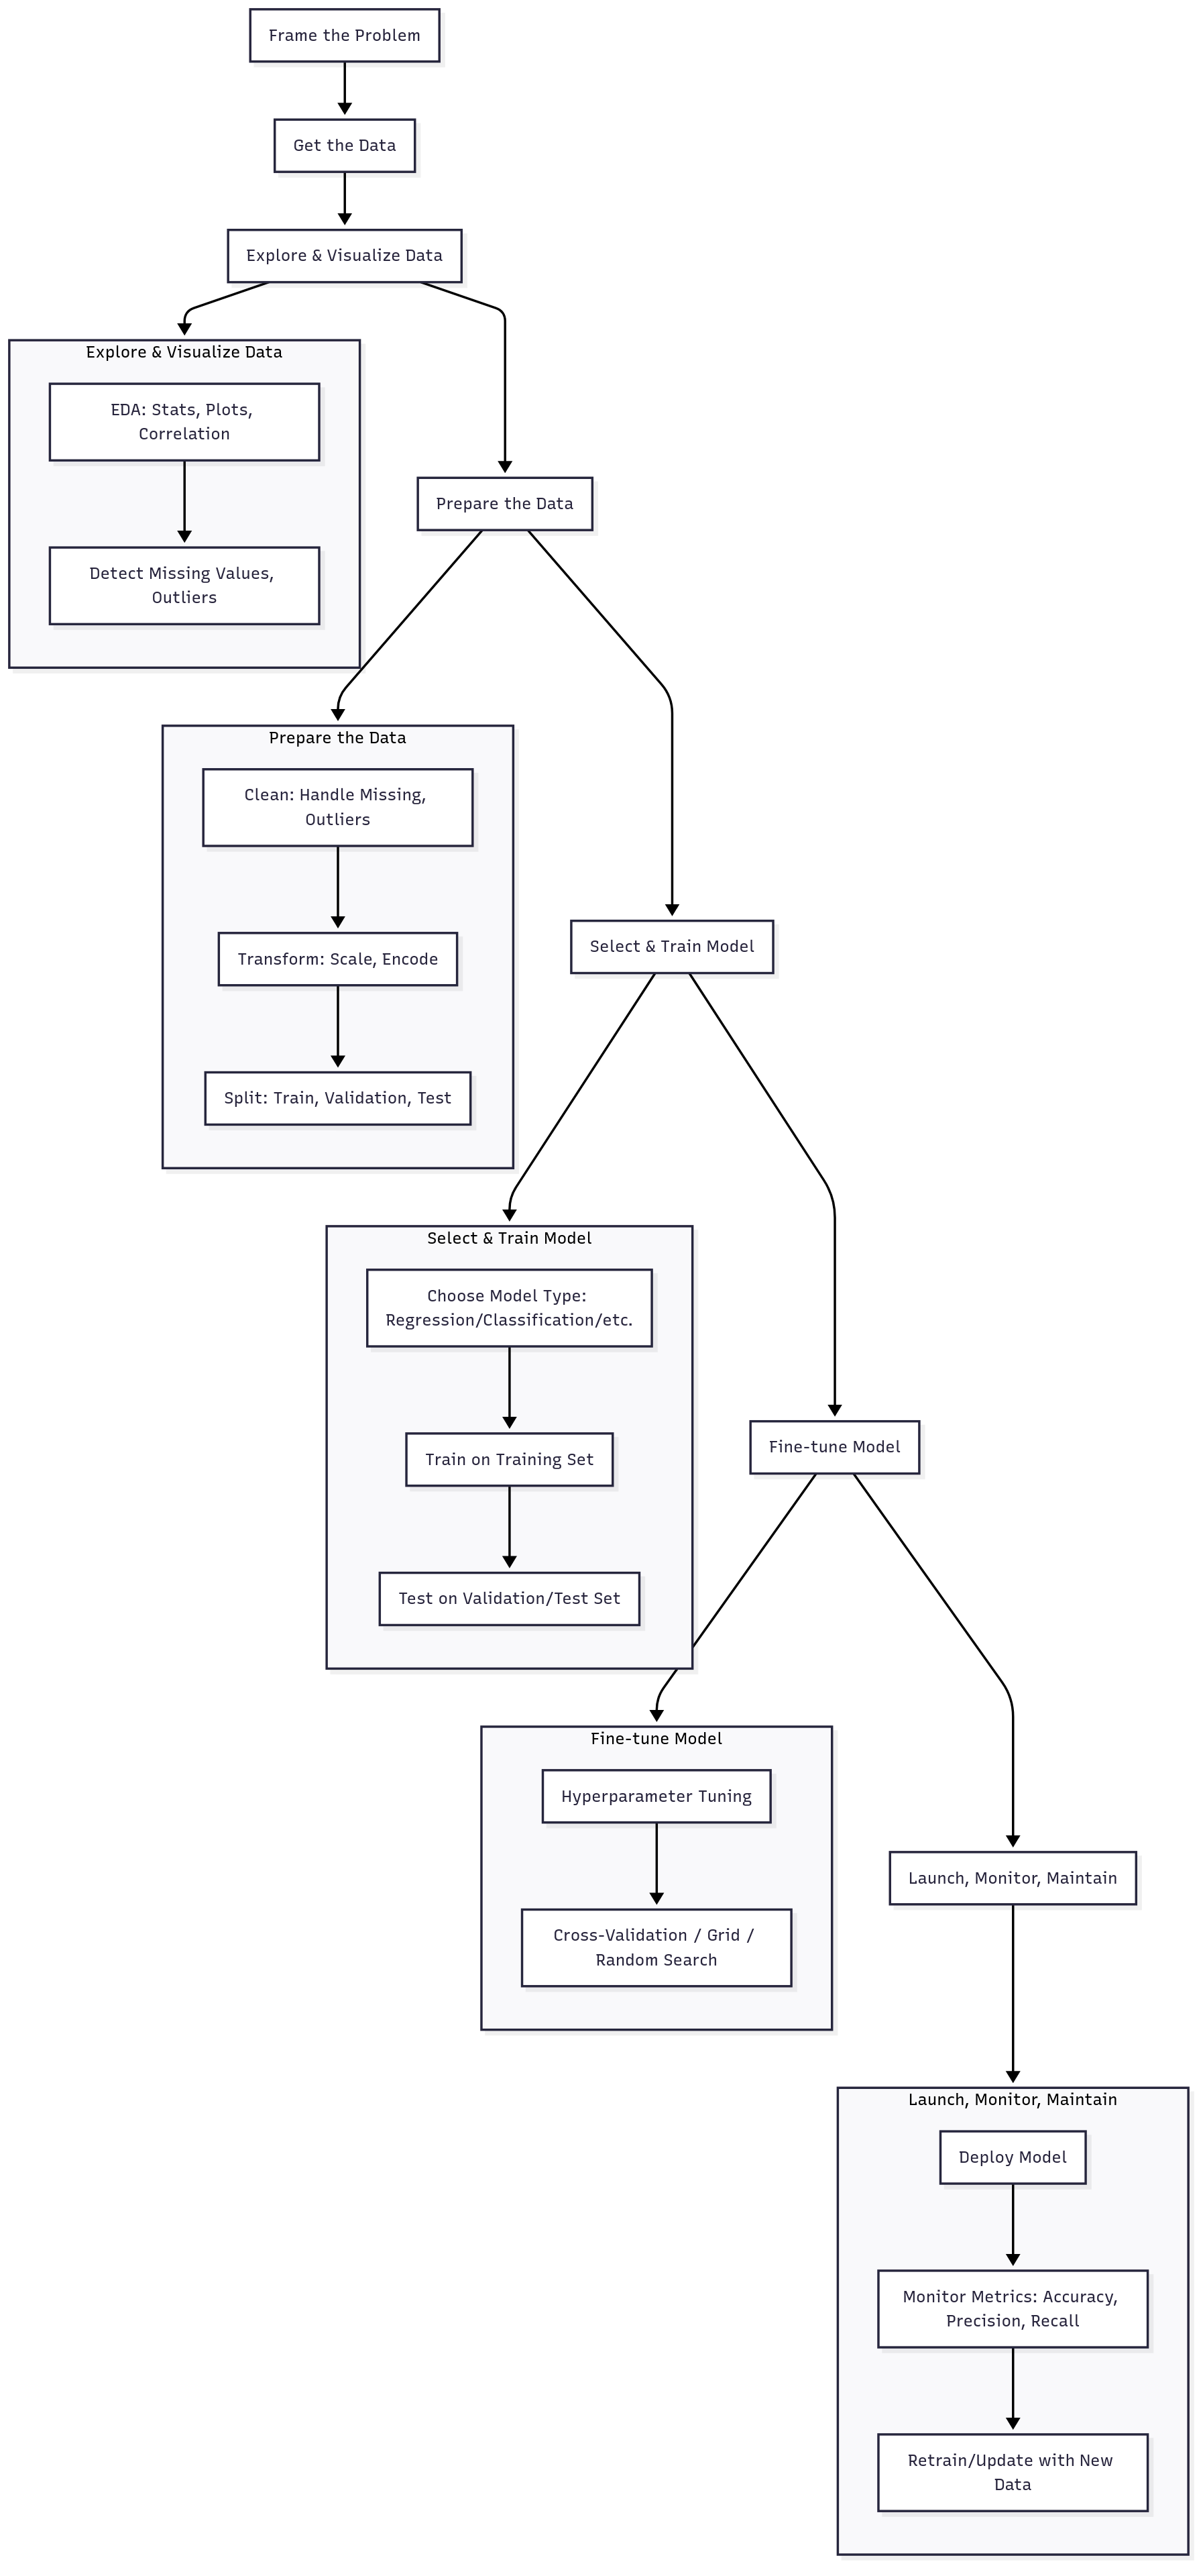
\includegraphics[width=0.8\textwidth]{chart.png}
    \caption{End-to-end machine learning project workflow}
    \label{fig:mlworkflow}
\end{figure}
\section{Conclusion}
In conclusion, an end-to-end machine learning project involves several key steps, including framing the problem, gathering and preparing the data, selecting and training a model, fine-tuning its hyperparameters, and deploying and maintaining the model in production. Each step is crucial to the success of the project,

\end{document}